% !TEX root = cha-soa.tex
\documentclass[../../main.tex]{subfiles}

\begin{document}

\subsection{Standard WFC}
\label{subsec:soa_standard_wfc}

Borrowing concepts and terminology from quantum mechanics, Wave Function Collapse (WFC) starts with a grid of cells, where each cell contains a set of possible tiles. This set represents the states that the cell can have before a final configuration is selected by the algorithm. A cell with multiple possible tiles is therefore said to be in a ``superposition'' state. The goal of WFC is to reduce these possibilities until every cell has been assigned to exactly one tile, while ensuring that all local constraints are satisfied.

WFC is based on two main components: a \emph{tileset} and a set of \emph{adjacency rules}. The tileset defines the elements in which a cell can be collapsed to, while the adjacency rules specify which tiles are compatible with each other along each direction. These components are defined differently depending on the model, leading to two variants:

\begin{itemize}
    \item \textbf{Tile-based model}: The tiles and their adjacency rules are manually defined by the user. Each tile has a set of compatible neighbors for each direction. This model provides direct control over both the elements that can be generated and their adjacency constraints. An example of the tile-based model from Gumin's GitHub repository~\citeonline{Gumin2016wfc} is shown in \figref{fig:wfc_tile_based}.

    \begin{figure}[h]
        \centering
        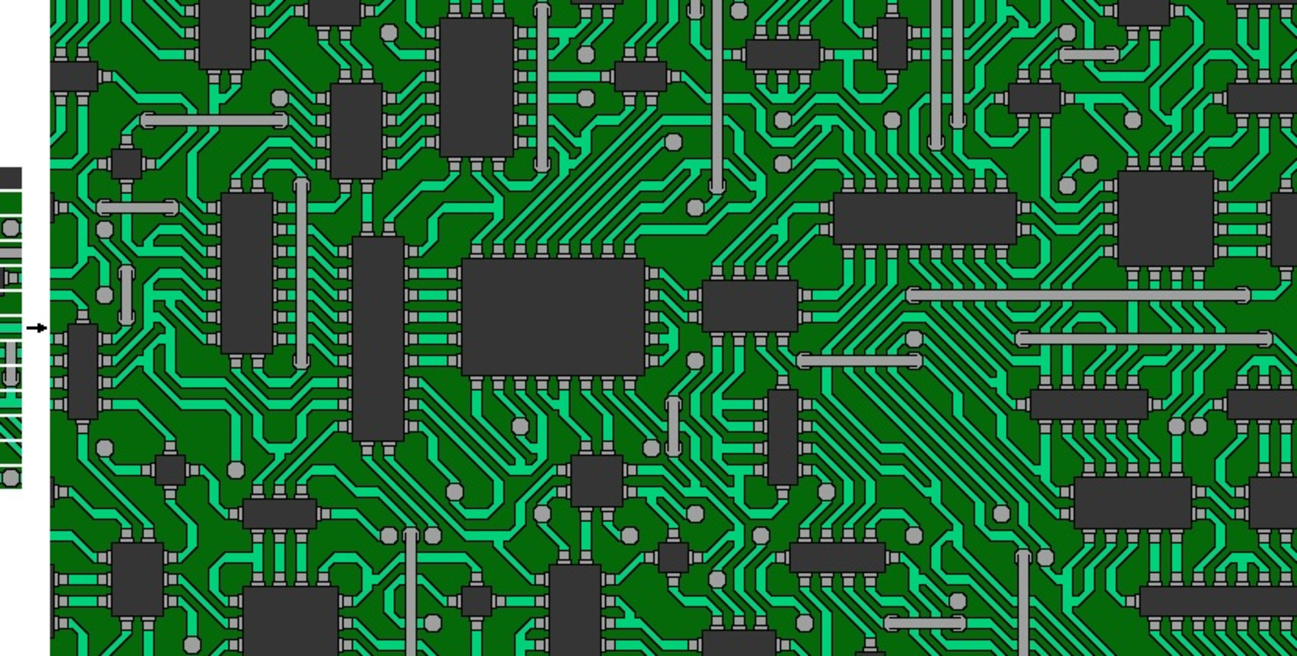
\includegraphics[width=0.9\linewidth]{figures/soa/tile-based_example}
        \caption{Example of tile-based model.}
        \label{fig:wfc_tile_based}
    \end{figure}

    \item \textbf{Overlapping model}: The tiles and their adjacency rules are extracted from an input example. This allows WFC to reproduce local patterns from the input while generating a new configuration. Some examples of the overlapping model from Gumin's GitHub repository~\citeonline{Gumin2016wfc} are shown in \figref{fig:wfc_overlapping}.

\end{itemize}

\begin{figure}[h]
    \centering
    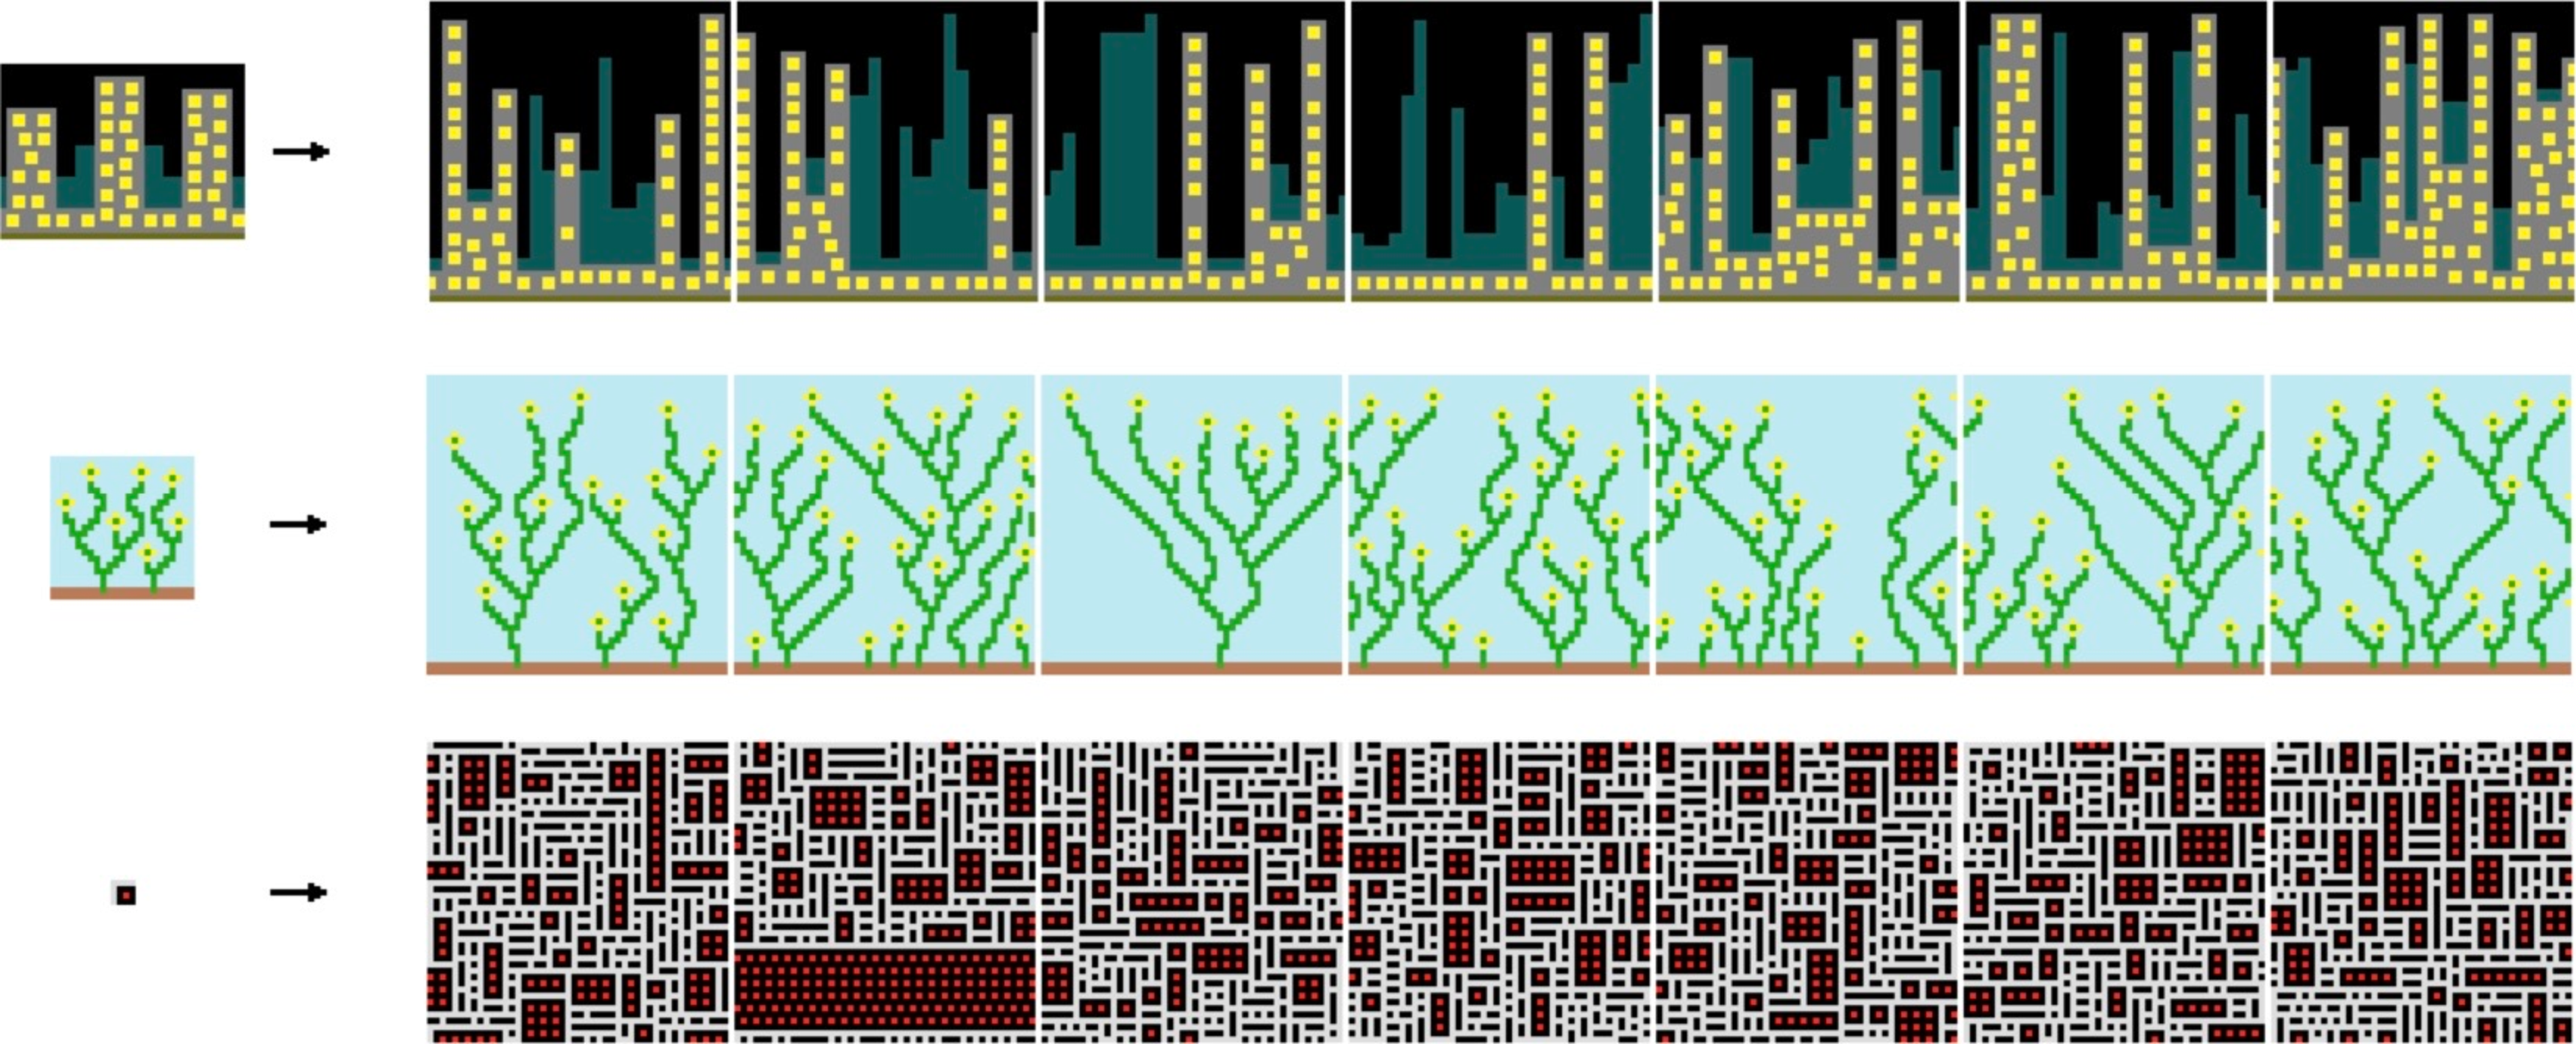
\includegraphics[width=0.9\linewidth]{figures/soa/overlapping_example}
    \caption{Examples of overlapping model.}
    \label{fig:wfc_overlapping}
\end{figure}

Regardless of the model, the generation process consists of two main phases: \emph{observation} and \emph{propagation}. The overall process is summarized in \algref{alg:wfc}.

\begin{algorithm}
    \caption{Wave Function Collapse}
    \label{alg:wfc}
        \begin{algorithmic}[1]
            \STATE Build possible tiles and constraint tables
            \STATE Initialize grid: cells in superposition of all possible tiles
            \REPEAT
                \STATE Choose next cell to collapse
                \STATE Collapse it to a tile
                \STATE Propagate the constraints
            \UNTIL{all cells are collapsed \OR no possible tiles for the selected cell remain}
        \end{algorithmic}
\end{algorithm}

\textbf{Initialization (Lines 1 and 2).}
The algorithm builds the tileset and the corresponding constraint tables. The grid is then initialized so that each cell contains the tiles that are initially allowed at that position. At this point, no cell has been assigned a final tile, and every cell is in a superposition state.

\textbf{Observation Phase (Lines 4 and 5).}
During the observation phase the algorithm selects an uncollapsed cell and reduces its state from a superposition of multiple potential tiles to a single, definite tile. The choice of cell can be guided by different heuristics~\citebibliography{Karth2022a}. A common strategy is to select the cell with the lowest entropy, corresponding to the cell with the least uncertainty. Other strategies include random selection, maximum entropy, and predefined orders such as left-to-right, spiral, or Hilbert curves.

Entropy can be defined simply as the number of remaining possible tiles. However, when at each tile is assigned a weight, Shannon entropy can be used. Given a set of possible tiles with weights $w_1, \ldots, w_n$, we first define the probability $p_i$ of picking tile $i$ by normalizing its weight over the sum of all remaining weights:

\begin{equation}
    p_i = \frac{w_i}{\sum_{j=1}^{n} w_j}
\end{equation}

The standard Shannon entropy $H$ of the cell is then expressed as:

\begin{equation}
    H = - \sum_{i=1}^{n} p_i \ln p_i\
\end{equation}

After selecting a cell, WFC chooses one of its possible tiles. This choice can also be guided by different strategies. A weighted strategy assigns different probabilities to the possible tiles, while other strategies can select random, rarest, or most common tile~\citebibliography{Karth2022a}.

As multiple tiles may be valid choices for a cell, different observations can lead to different configurations. WFC is therefore inherently non-deterministic: running the same instance multiple times can produce different outputs while satisfying the same set of constraints.

\textbf{Propagation Phase (Line 6).} Once a cell is collapsed, the algorithm propagates the information to its uncollapsed neighbors verifying the constraints and reducing their remaining tiles accordingly. For each neighbor, any tile that is no longer compatible with the tile of the collapsed cell is removed from its tileset. If this removal reduces the candidates of a neighbor, the information is recursively propagated. This continues until no more candidates are eliminated from any cell. 

If a cell reaches an empty set of candidate tiles, a contradiction has occurred, the current attempt is invalid, and the algorithm stops. In this case, the standard implementation by Gumin does not perform backtracking. Instead, the current generation attempt is discarded, and the algorithm starts again from the initial state. If repeated attempts fail to produce a valid configuration, the generation is considered unsuccessful. 

Other WFC variants can introduce backtracking to recover from contradictions without restarting the entire generation. In this case, the algorithm can restore a previously saved state and make different choices from that point onward, relying on the fact that a different sequence of collapses may lead to a valid solution.

In \figref{fig:step-explanation}, we show a step of the main loop in the WFC algorithm (observation and propagation phases).

\begin{figure}[ht] 
   \centering 
   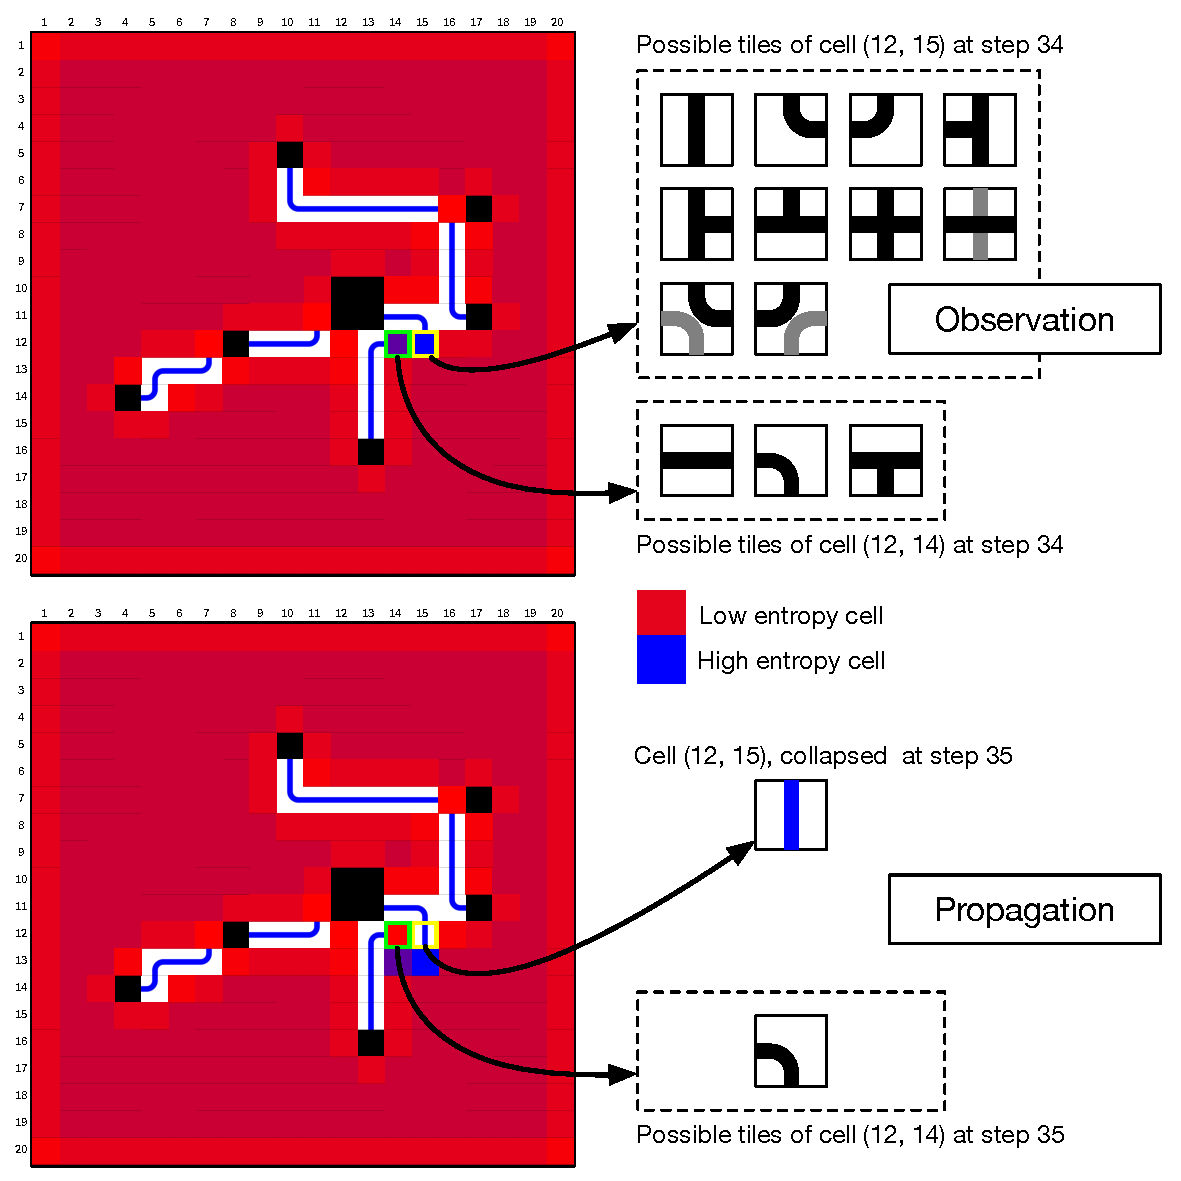
\includegraphics[width=0.85\linewidth]{figures/soa/step-explanation} 
   \caption{Example of one iteration step of the main WFC loop. \SL{Aggiorna con il gradiente}}
 \label{fig:step-explanation}
\end{figure}

\end{document}